%\clearpage

\section{Results}
\label{sec:results}

\subsection{Background estimate from the ABCD method}
\label{sec:abcdres}

The data yields in the 
four regions are summarized in Tables~\ref{tab:datayield1}-Table~\ref{tab:datayield3}
for the 3 signal regions.

\newpage


\begin{figure}[tbh]
\begin{center}
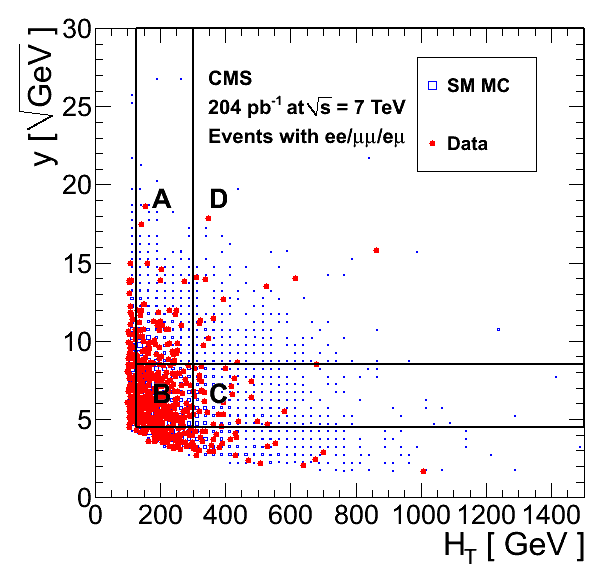
\includegraphics[width=0.75\linewidth]{plots/abcd_204pb_2010.png}
\caption{\label{fig:abcdData1}\protect Distributions of $y$ 
vs. \Ht for SM Monte Carlo and data. The 2010 signal region boundaries are overlayed.}
\end{center}
\end{figure}

\begin{table}[hbt]
\begin{center}
\caption{\label{tab:datayield1} Data yields in the four
regions of Figure~\ref{fig:abcdData1} for the 2010 signal region, 
as well as the predicted yield in region D given
by A $\times$ C / B.  The quoted uncertainty
on the prediction in data is statistical only, assuming Gaussian errors.
We also show the SM Monte Carlo expectations.}
\begin{tabular}{l||c|c|c|c||c}
\hline
           sample  &                A  &                B  &                C  &                D  &   A $\times$ B / C  \\
\hline
           \ttbar  & 48.8  $\pm$  1.4  &184.1  $\pm$  2.7  & 31.9  $\pm$  1.1  &  7.3  $\pm$  0.5  &  8.5  $\pm$  0.4    \\
               DY  &  0.5  $\pm$  0.4  &  8.2  $\pm$  1.5  &  0.7  $\pm$  0.5  &  1.0  $\pm$  0.6  &  0.0  $\pm$  0.0    \\
              \WW  &  0.6  $\pm$  0.1  &  1.6  $\pm$  0.1  &  0.1  $\pm$  0.0  &  0.2  $\pm$  0.0  &  0.1  $\pm$  0.0    \\
              \WZ  &  0.1  $\pm$  0.0  &  0.3  $\pm$  0.0  &  0.0  $\pm$  0.0  &  0.0  $\pm$  0.0  &  0.0  $\pm$  0.0    \\
              \ZZ  &  0.0  $\pm$  0.0  &  0.1  $\pm$  0.0  &  0.0  $\pm$  0.0  &  0.0  $\pm$  0.0  &  0.0  $\pm$  0.0    \\
       single top  &  1.9  $\pm$  0.1  &  5.6  $\pm$  0.2  &  0.2  $\pm$  0.0  &  0.1  $\pm$  0.0  &  0.1  $\pm$  0.0    \\
           \wjets  &  0.6  $\pm$  0.6  &  1.2  $\pm$  0.6  &  0.0  $\pm$  0.0  &  0.0  $\pm$  0.0  &  0.0  $\pm$  0.0    \\
\hline
      Total SM MC  & 52.6  $\pm$  1.6  &201.2  $\pm$  3.2  & 33.1  $\pm$  1.2  &  8.6  $\pm$  0.8  &  8.6  $\pm$  0.4    \\
\hline
             data  &               72  &              238  &               29  &               14  &  8.8  $\pm$  2.0    \\
\hline
\end{tabular}
\end{center}
\end{table}

\newpage

\begin{figure}[tbh]
\begin{center}
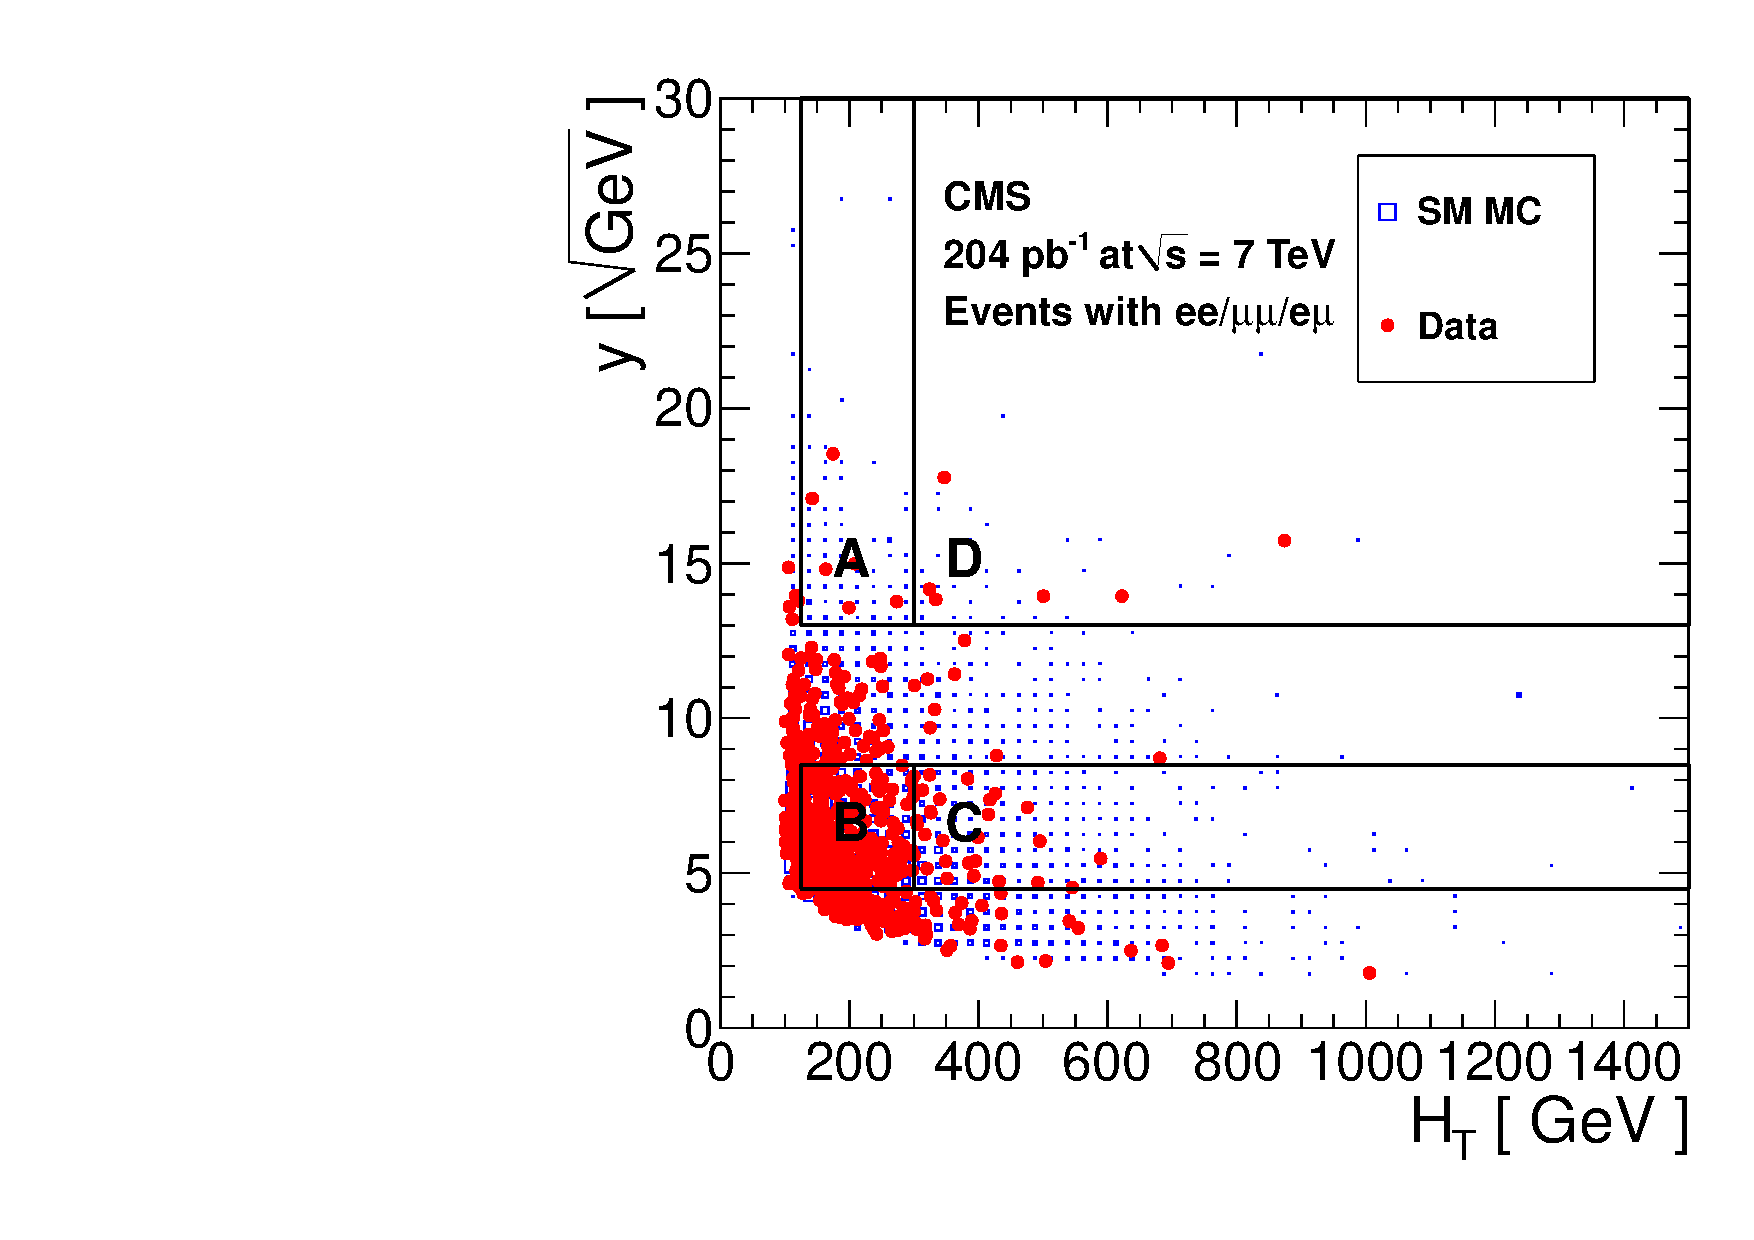
\includegraphics[width=0.75\linewidth]{plots/abcd_204pb_highy.pdf}
\caption{\label{fig:abcdData2}\protect Distributions of $y$ 
vs. \Ht for SM Monte Carlo and data. The high $y$ signal region boundaries are overlayed.}
\end{center}
\end{figure}


\begin{table}[hbt]
\begin{center}
\caption{\label{tab:datayield2} Data yields in the four
regions of Figure~\ref{fig:abcdData2} for the high $y$ signal region, 
as well as the predicted yield in region D given
by A $\times$ C / B.  The quoted uncertainty
on the prediction in data is statistical only, assuming Gaussian errors.
We also show the SM Monte Carlo expectations.}
\begin{tabular}{l||c|c|c|c||c}
\hline
           sample  &                A  &                B  &                C  &                D  &   A $\times$ B / C   \\
\hline
           \ttbar  &  3.6  $\pm$  0.4  &184.1  $\pm$  2.7  & 31.9  $\pm$  1.1  &  1.2  $\pm$  0.2  &  0.6  $\pm$  0.1  \\
               DY  &  0.3  $\pm$  0.3  &  8.2  $\pm$  1.5  &  0.7  $\pm$  0.5  &  0.0  $\pm$  0.0  &  0.0  $\pm$  0.0  \\
              \WW  &  0.1  $\pm$  0.0  &  1.6  $\pm$  0.1  &  0.1  $\pm$  0.0  &  0.1  $\pm$  0.0  &  0.0  $\pm$  0.0  \\
              \WZ  &  0.0  $\pm$  0.0  &  0.3  $\pm$  0.0  &  0.0  $\pm$  0.0  &  0.0  $\pm$  0.0  &  0.0  $\pm$  0.0  \\
              \ZZ  &  0.0  $\pm$  0.0  &  0.1  $\pm$  0.0  &  0.0  $\pm$  0.0  &  0.0  $\pm$  0.0  &  0.0  $\pm$  0.0  \\
       single top  &  0.2  $\pm$  0.0  &  5.6  $\pm$  0.2  &  0.2  $\pm$  0.0  &  0.0  $\pm$  0.0  &  0.0  $\pm$  0.0  \\
           \wjets  &  0.0  $\pm$  0.0  &  1.2  $\pm$  0.6  &  0.0  $\pm$  0.0  &  0.0  $\pm$  0.0  &  0.0  $\pm$  0.0  \\
\hline
      Total SM MC  &  4.1  $\pm$  0.5  &201.2  $\pm$  3.2  & 33.1  $\pm$  1.2  &  1.3  $\pm$  0.2  &  0.7  $\pm$  0.1  \\
\hline
             data  &                6  &              238  &               29  &                6  &  0.7  $\pm$  0.3  \\
\hline
\end{tabular}
\end{center}
\end{table}

\newpage

\begin{figure}[tbh]
\begin{center}
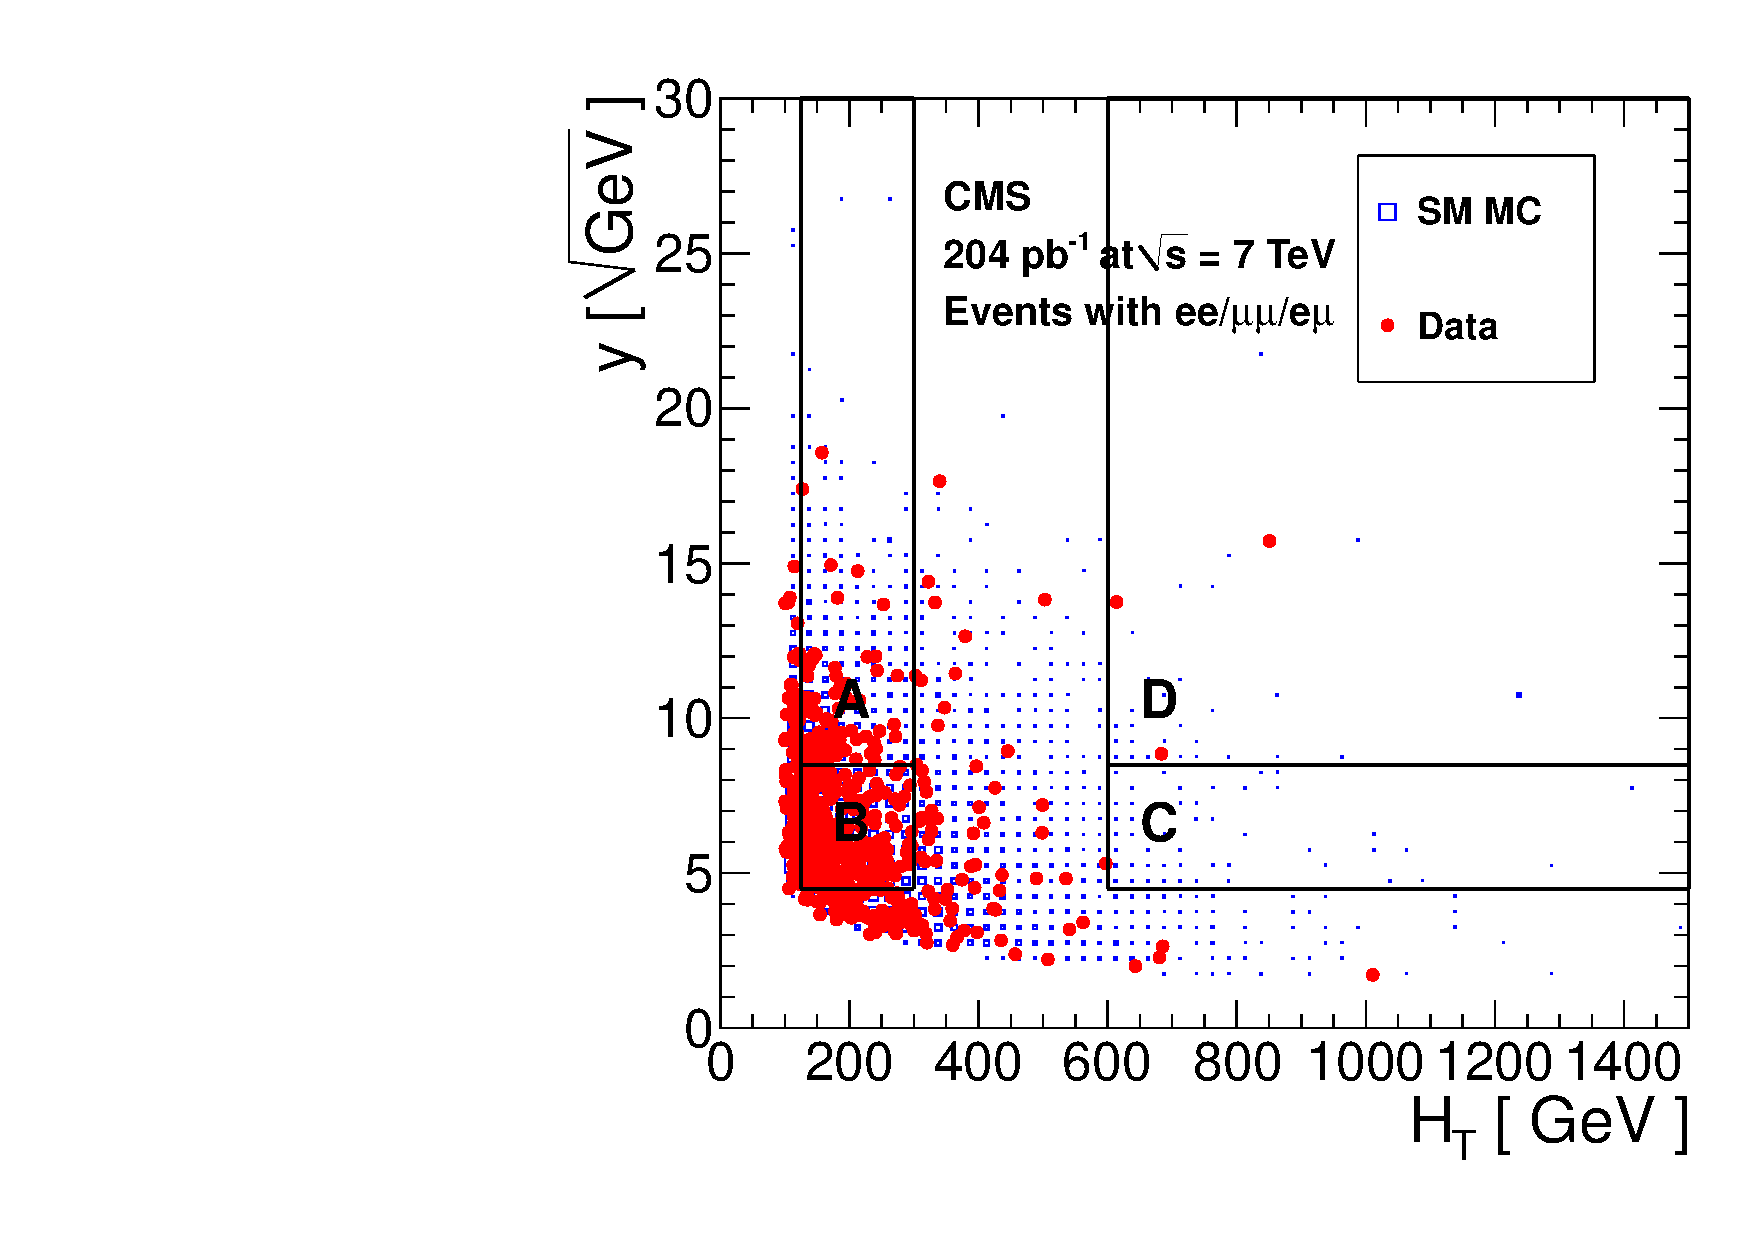
\includegraphics[width=0.75\linewidth]{plots/abcd_204pb_highht.pdf}
\caption{\label{fig:abcdData3}\protect Distributions of $y$ 
vs. \Ht for SM Monte Carlo and data. The high \Ht\ signal region boundaries are overlayed.}
\end{center}
\end{figure}

\begin{table}[hbt]
\begin{center}
\caption{\label{tab:datayield3} Data yields in the four
regions of Figure~\ref{fig:abcdData} for the high \Ht signal region, 
as well as the predicted yield in region D given
by A $\times$ C / B.  The quoted uncertainty
on the prediction in data is statistical only, assuming Gaussian errors.
Since the yield in region C is 0, we assess as the uncertainty the prediction
corresponding to 1 observed event in 1.
We also show the SM Monte Carlo expectations.}
\begin{tabular}{l||c|c|c|c||c}
\hline
           sample  &                A  &                B  &                C  &                D  &   A $\times$ B / C  \\
\hline
            ttall  & 48.8  $\pm$  1.4  &184.1  $\pm$  2.7  &  2.2  $\pm$  0.3  &  0.7  $\pm$  0.2  &  0.6  $\pm$  0.1   \\
               DY  &  0.5  $\pm$  0.4  &  8.2  $\pm$  1.5  &  0.0  $\pm$  0.0  &  0.4  $\pm$  0.4  &  0.0  $\pm$  0.0   \\
               WW  &  0.6  $\pm$  0.1  &  1.6  $\pm$  0.1  &  0.0  $\pm$  0.0  &  0.0  $\pm$  0.0  &  0.0  $\pm$  0.0   \\
               WZ  &  0.1  $\pm$  0.0  &  0.3  $\pm$  0.0  &  0.0  $\pm$  0.0  &  0.0  $\pm$  0.0  &  0.0  $\pm$  0.0   \\
               ZZ  &  0.0  $\pm$  0.0  &  0.1  $\pm$  0.0  &  0.0  $\pm$  0.0  &  0.0  $\pm$  0.0  &  0.0  $\pm$  0.0   \\
                t  &  1.9  $\pm$  0.1  &  5.6  $\pm$  0.2  &  0.0  $\pm$  0.0  &  0.0  $\pm$  0.0  &  0.0  $\pm$  0.0   \\
            wjets  &  0.6  $\pm$  0.6  &  1.2  $\pm$  0.6  &  0.0  $\pm$  0.0  &  0.0  $\pm$  0.0  &  0.0  $\pm$  0.0   \\
\hline
      Total SM MC  & 52.6  $\pm$  1.6  &201.2  $\pm$  3.2  &  2.2  $\pm$  0.3  &  1.2  $\pm$  0.5  &  0.6  $\pm$  0.1   \\
\hline
             data  &               72  &              238  &                0  &                3  &  0.0  $\pm$  0.3   \\
\hline
\end{tabular}
\end{center}
\end{table}






%\clearpage

\subsection{Background estimate from the $P_T(\ell\ell)$ method}
\label{sec:victoryres}

We first use the $P_T(\ell \ell)$ method to predict the number of events 
in control region A, defined in Sec.~\ref{sec:abcd} as 
$125<{\rm SumJetPt}>300$~GeV and $\met/\sqrt{\rm SumJetPt}>$8.5~GeV$^{1/2}$.
We count the number of events in region
$A'$, defined in Sec.~\ref{sec:othBG} by replacing the above $\met/\sqrt{\rm SumJetPt}$
cut with the same cut on the quantity $P_T(\ell\ell)/\sqrt{\rm SumJetPt}$,
and find $N_{A'}=5$. We subtract off the expected DY contribution in this region
$N_{DY} = 1.3 \pm 0.9$, derived in Sec.~\ref{sec:othBG}.
To predict the yield in region A we take 
$N_A = K \cdot K_C \cdot ( N_{A'} - N_{DY} ) = 9.0 \pm 6.0$
where we have taken $K = 1.7$ and $K_C = 1.4$.
This uncertainty takes into account the statistical uncertainties in $N_{A'}$ and $N_{DY}$,
assuming Gaussian errors. This yield is consistent
with the observed yield of 12 events, as shown in 
Table~\ref{tab:victory} and displayed in Fig.~\ref{fig:victory} (left).

Encouraged by the good agreement between predicted and observed yields
in the control region, we proceed to perform the $P_T(\ell \ell)$ method 
in the signal region ${\rm SumJetPt}>300$~GeV.
The number of data events in region $D'$, which is defined in 
Section~\ref{sec:othBG} to be the same as region $D$ but with the
$\met/\sqrt{\rm SumJetPt}$ requirement 
replaced by a $P_T(\ell\ell)/\sqrt{\rm SumJetPt}$ requirement,
is $N_{D'}=1$.  
%We next subtract off the expected DY contribution of 
%$N_{DY}$ = $0.4 \pm 0.4$ events, as calculated 
%in Sec.~\ref{sec:othBG}. 
The BG prediction is 
$N_D = K \cdot K_C \cdot (N_{D'}-N_{DY}) = 2.1 \pm 2.1({\rm stat}) \pm 0.6({\rm syst})$ 
where $K=1.5$ as derived in Sec.~\ref{sec:victory} and $K_C = 1.4 \pm 0.4$.
This prediction is consistent with the observed yield of 1 event, as summarized 
in Table~\ref{tab:victory} and Fig.~\ref{fig:victory} (right).


\begin{figure}[hbt]
\begin{center}
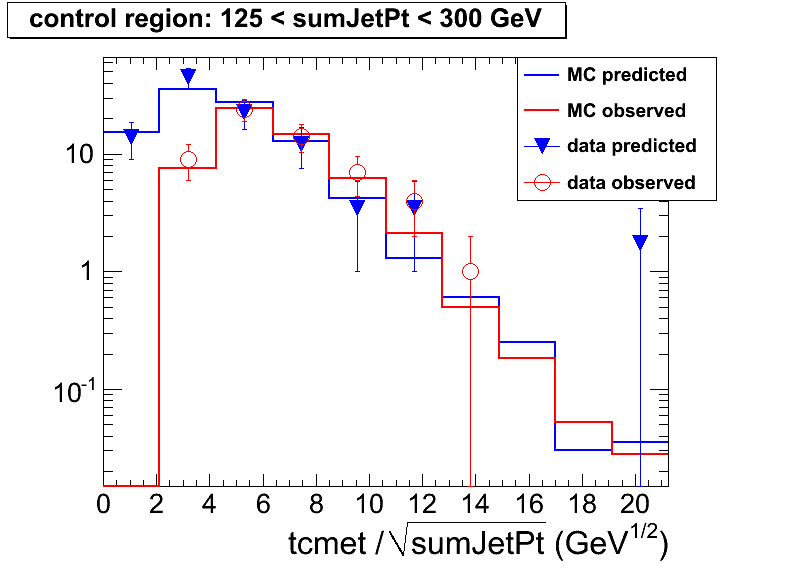
\includegraphics[width=0.48\linewidth]{victory_control_jsonv3.png}
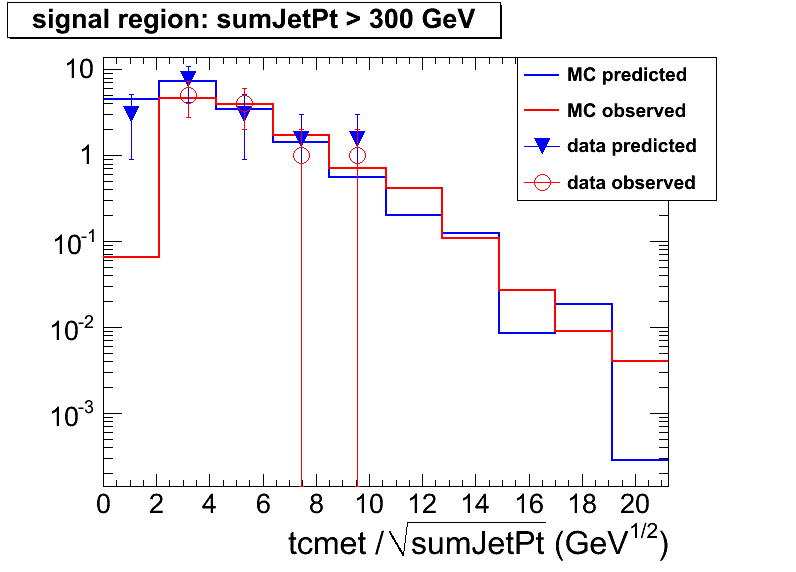
\includegraphics[width=0.48\linewidth]{victory_signal_jsonv3.png}
\caption{\label{fig:victory}\protect Distributions of 
tcMet/$\sqrt{\rm SumJetPt}$ for the control and signal region.
We show the oberved distributions in both Monte Carlo and data.
We also show the distributions predicted from 
${P_T(\ell\ell)}/\sqrt{\rm SumJetPt}$ in both MC and data.}
\end{center}
\end{figure}


\begin{table}[hbt]
\begin{center}
\caption{\label{tab:victory}Results of the dilepton $p_{T}$ template method in the control region
($125 < \mathrm{SumJetPt} < 300$~GeV) and signal region ($\mathrm{SumJetPt} > 300$~GeV). The predicted and 
observed yields for the region $\mathrm{tcmet}/\sqrt{\mathrm{sumJetPt}} > 8.5$~GeV$^{1/2}$. The errors are
statistical only, assuming Gaussian errors. Note that the correction factor $K_C$ has been applied to
the data but not to the MC.  }
\begin{tabular}{l|cc|cc}
\hline
              &    Control Region   &                        &   Signal Region    &               \\
\hline
              & Predicted           &   Observed             &   Predicted        &  Observed     \\              
\hline
total SM   MC &      6.45           &       9.14             &   0.92             &  1.27         \\
         data &  $9.0 \pm 6.0$      &         12             &   $2.1 \pm 2.1$    &  1            \\
\hline
\end{tabular}
\end{center}
\end{table}



% \clearpage
\subsection{Summary of results}

In summary, in the signal region defined as $\mathrm{SumJetPt}>300$~GeV and $\met/\sqrt{\rm SumJetPt} > 8.5$~GeV$^{1/2}$:\\ 
We observe 1 event. \\
We expect 1.3 events from Standard Model MC prediction. \\
The ABCD data driven method predicts $1.3 \pm 0.8({\rm stat}) \pm 0.3({\rm syst})$ events. \\
The  $P_T(\ell\ell)$ method predicts $2.1 \pm 2.1({\rm stat}) \pm 0.6({\rm syst})$ events. \\
  
All three background estimates are consistent within their uncertainties.
We thus take as our best estimate of the Standard Model yield in 
the signal region the average of the predicted yields from the 2 data-driven methods, 
weighted by their uncertainties.
This procedure gives an expected background yield $N_{BG}=1.4 \pm 0.8$.

We conclude that we see no evidence for an anomalous 
rate of opposite sign isolated dilepton events
at high \met and high SumJetPt.  The extraction of 
quantitative limits on new physics models is discussed
in Section~\ref{sec:limit}.
